
\documentclass[final]{beamer}

\usepackage[scale=1.24]{beamerposter} % Use the beamerposter package for laying out the poster

\usetheme{confposter} % Use the confposter theme supplied with this template

\setbeamercolor{block title}{fg=ngreen,bg=white} % Colors of the block titles
\setbeamercolor{block body}{fg=black,bg=white} % Colors of the body of blocks
\setbeamercolor{block alerted title}{fg=white,bg=dblue!70} % Colors of the highlighted block titles
\setbeamercolor{block alerted body}{fg=black,bg=dblue!10} % Colors of the body of highlighted blocks
% Many more colors are available for use in beamerthemeconfposter.sty

%-----------------------------------------------------------
% Define the column widths and overall poster size
% To set effective sepwid, onecolwid and twocolwid values, first choose how many columns you want and how much separation you want between columns
% In this template, the separation width chosen is 0.024 of the paper width and a 4-column layout
% onecolwid should therefore be (1-(# of columns+1)*sepwid)/# of columns e.g. (1-(3+1)*0.025)/3 = 0.3
% Set twocolwid to be (2*onecolwid)+sepwid = 0.625

\newlength{\sepwid}
\newlength{\onecolwid}
\newlength{\twocolwid}
\setlength{\paperwidth}{48in} % A0 width: 46.8in
\setlength{\paperheight}{36in} % A0 height: 33.1in
\setlength{\sepwid}{0.025\paperwidth} % Separation width (white space) between columns
\setlength{\onecolwid}{0.3\paperwidth} % Width of one column
\setlength{\twocolwid}{0.625\paperwidth} % Width of two columns
\setlength{\topmargin}{-0.5in} % Reduce the top margin size
%-----------------------------------------------------------

\usepackage{graphicx}  % Required for including images

\usepackage{booktabs} % Top and bottom rules for tables

%----------------------------------------------------------------------------------------
%	TITLE SECTION 
%----------------------------------------------------------------------------------------

\title{A DeepRL Framework for Robot Locomotion in Complex environments} % Poster title

\author{Msc.(c) Wilbert Pumacay Huallpa} % Author(s)
\institute{Catholic University San Pablo - wilbert.pumacay@ucsp.edu.pe} % Institution(s)
%----------------------------------------------------------------------------------------

\begin{document}

\addtobeamertemplate{block end}{}{\vspace*{2ex}} % White space under blocks
\addtobeamertemplate{block alerted end}{}{\vspace*{2ex}} % White space under highlighted (alert) blocks

\setlength{\belowcaptionskip}{2ex} % White space under figures
\setlength\belowdisplayshortskip{2ex} % White space under equations

\begin{frame}[t] % The whole poster is enclosed in one beamer frame

\begin{columns}[t] % The whole poster consists of three major columns, the second of which is split into two columns twice - the [t] option aligns each column's content to the top

\begin{column}{\sepwid}\end{column} % Empty spacer column

\begin{column}{\onecolwid} % The first column

%----------------------------------------------------------------------------------------
%	PROBLEM STATEMENT
%----------------------------------------------------------------------------------------

\begin{block}{Problem Statement}

    \begin{itemize}
        \item \textbf{Learning Environments} are a key part of RL research (e.g. ALE[1]).
        \item \textbf{Performance over wide range of environments} is a good measure for intelligence[2].
            \begin{equation*}
                \Upsilon (\pi) = \Sigma_{\mu \in E} 2^{-K(\mu)} V^{\pi}_{\mu}
            \end{equation*}
        \item \textbf{Current locomotion benchmarks} provide low to middle level complex tasks, like in [3], [4].
    \end{itemize}

\end{block}

%----------------------------------------------------------------------------------------
%	RELATED WORKS
%----------------------------------------------------------------------------------------

\begin{block}{Related Works}

\end{block}

\begin{figure}
	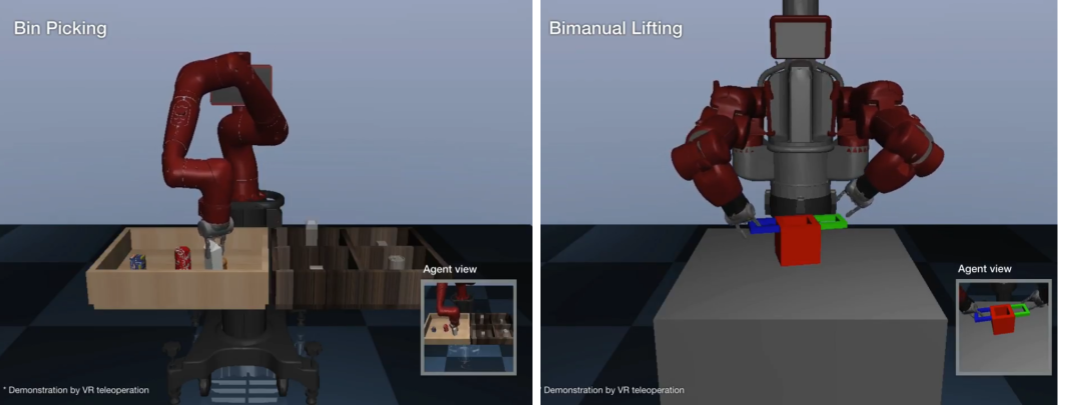
\includegraphics[width=0.8\linewidth]{_imgs/img_related_works_surreal.png}
	\caption{SURREAL[5]}
\end{figure}

\begin{figure}
    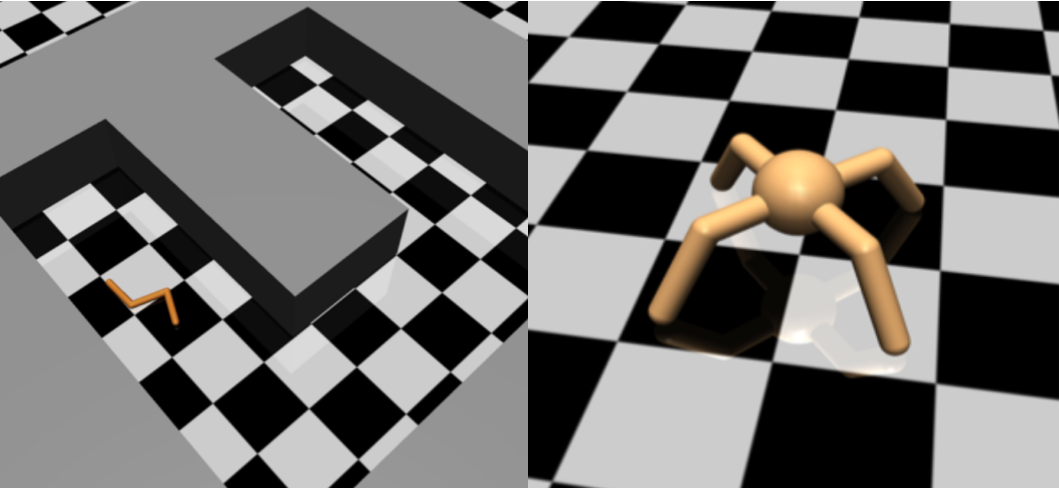
\includegraphics[width=0.8\linewidth]{_imgs/img_related_works_rllab.png}
    \caption{RLlab [6]}
\end{figure}

\begin{figure}
	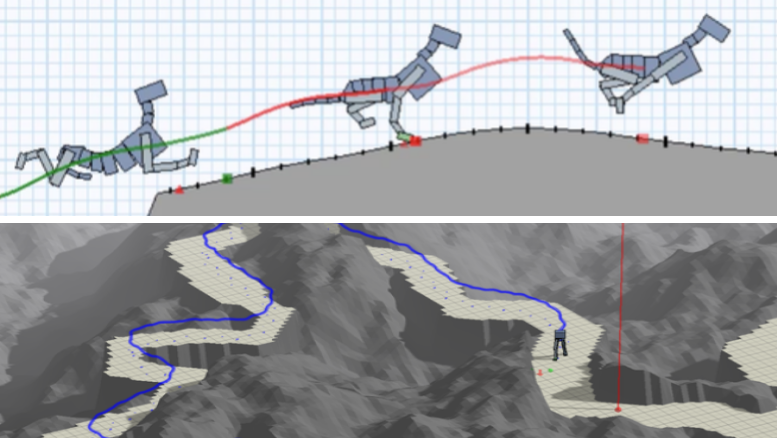
\includegraphics[width=0.8\linewidth,height=0.3\linewidth]{_imgs/img_related_works_terrainrlsim.png}
	\caption{TerrainRLSim [4]}
\end{figure}

%----------------------------------------------------------------------------------------

\end{column} % End of the first column
\begin{column}{\sepwid}\end{column} % Empty spacer column

\begin{column}{\onecolwid} % Begin a column which is two columns wide (column 2)

\begin{block}{Approach}

    \begin{itemize}
        \item \textbf{Close to the backend}: the framework is written in C++
                close to the physics and graphics backends.
        \item \textbf{But not that close}: the core framework in designed to be
                agnostic of the physics and graphics backends to allow easy integration
                into your backends of choice.
        \item \textbf{Any-environment}: the framework is designed to allow the
                creation of lots of environments easily by means of utilities on top.
        \item \textbf{Python API}: the underlying framework is written in C++,
                with a Python API on top that exposes to the user the necessary functionality
                to create environments, define tasks, create agents and sensors, etc.
    \end{itemize}

    \begin{figure}
        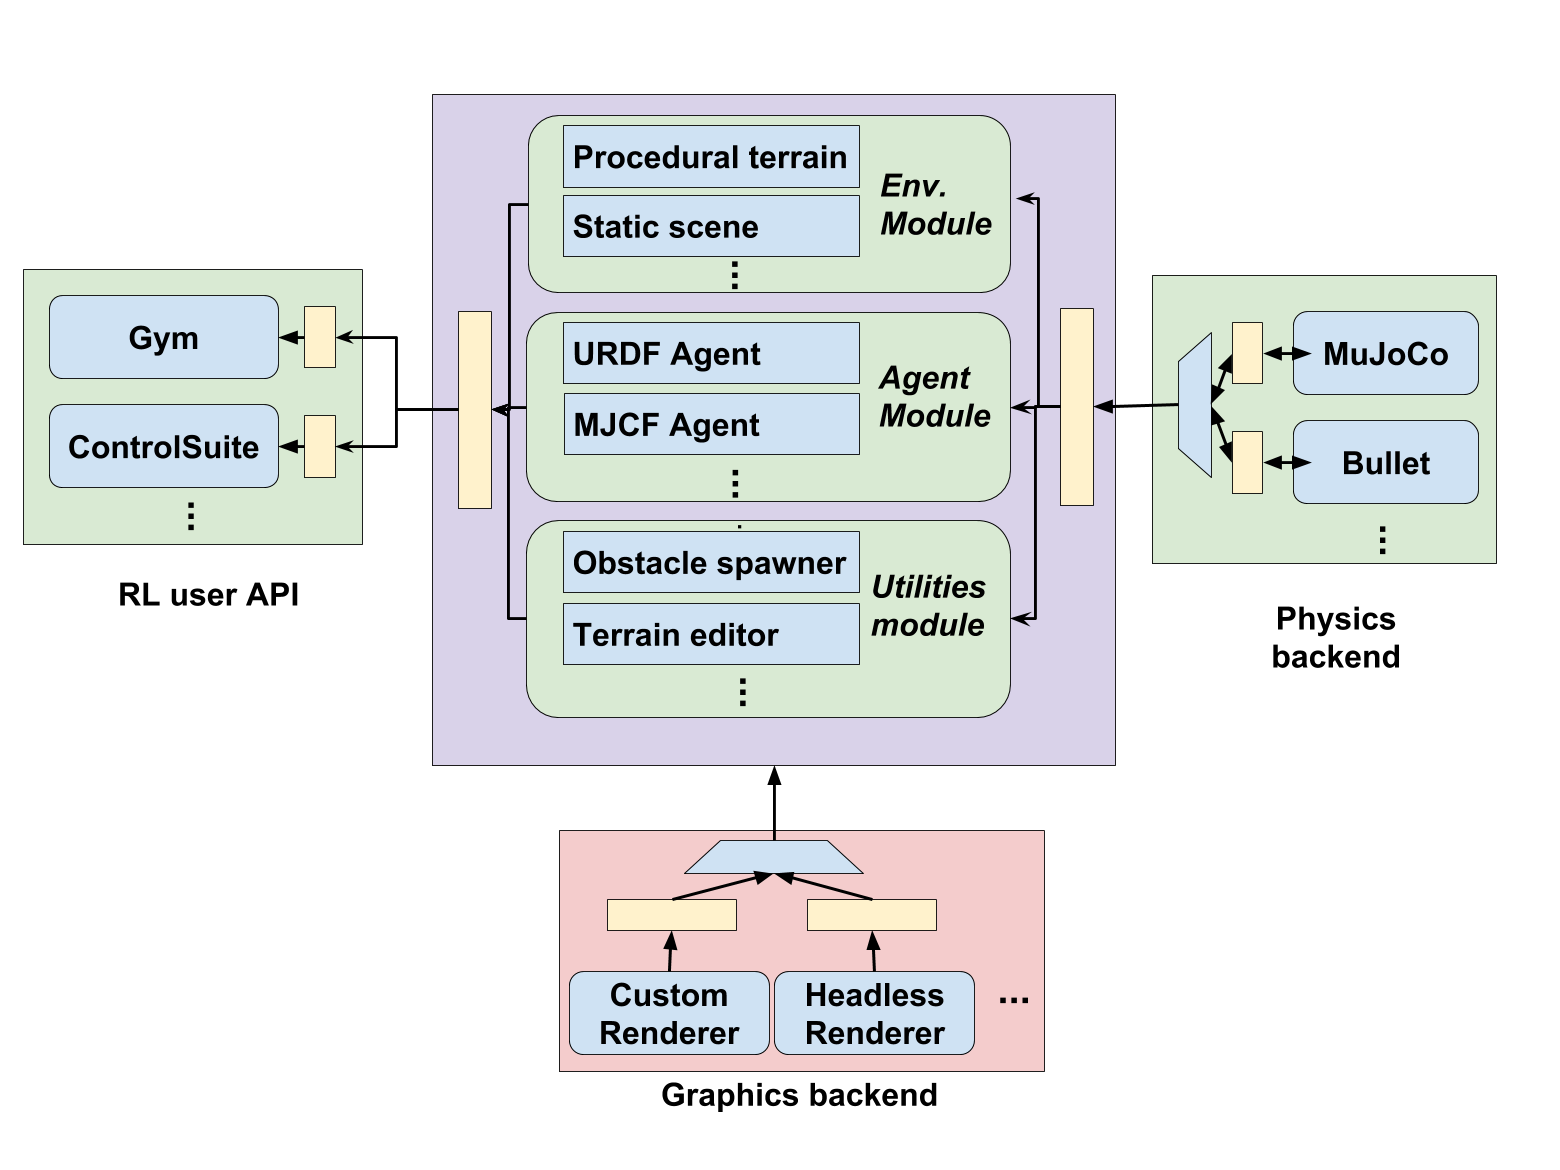
\includegraphics[width=0.85\linewidth]{_imgs/img_proposed_framework.png}
        \caption{Framework Overview}
    \end{figure}

\end{block}

\begin{block}{Current Progress}

    \begin{figure}
        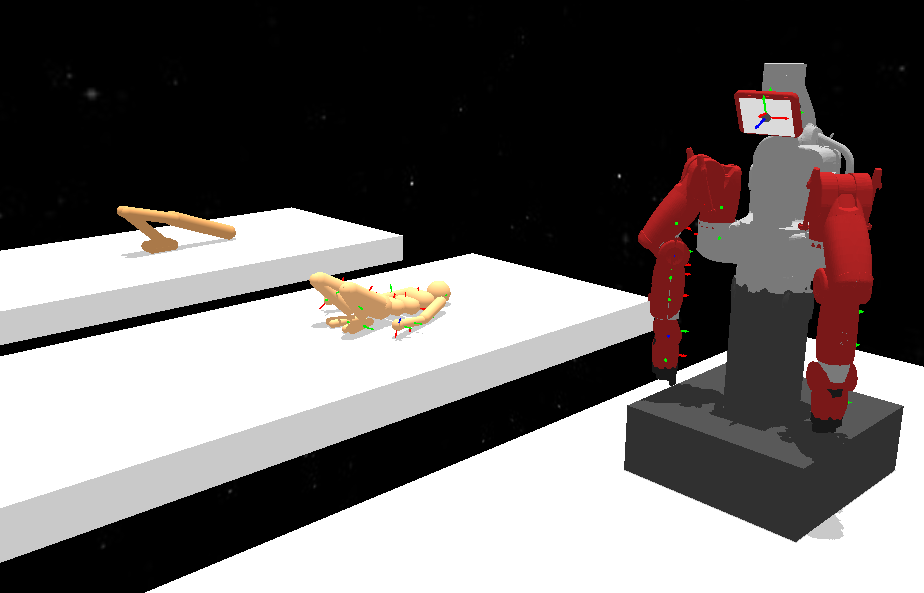
\includegraphics[width=0.8\linewidth]{_imgs/img_tysocmjc_agents_1.png}
        \caption{Agents}
    \end{figure}

\end{block}

\begin{column}{\sepwid}\end{column} % Empty spacer column
\end{column} % End of the first column

\begin{column}{\sepwid}\end{column} % Empty spacer column
\begin{column}{\onecolwid} % The third column

\begin{figure}
    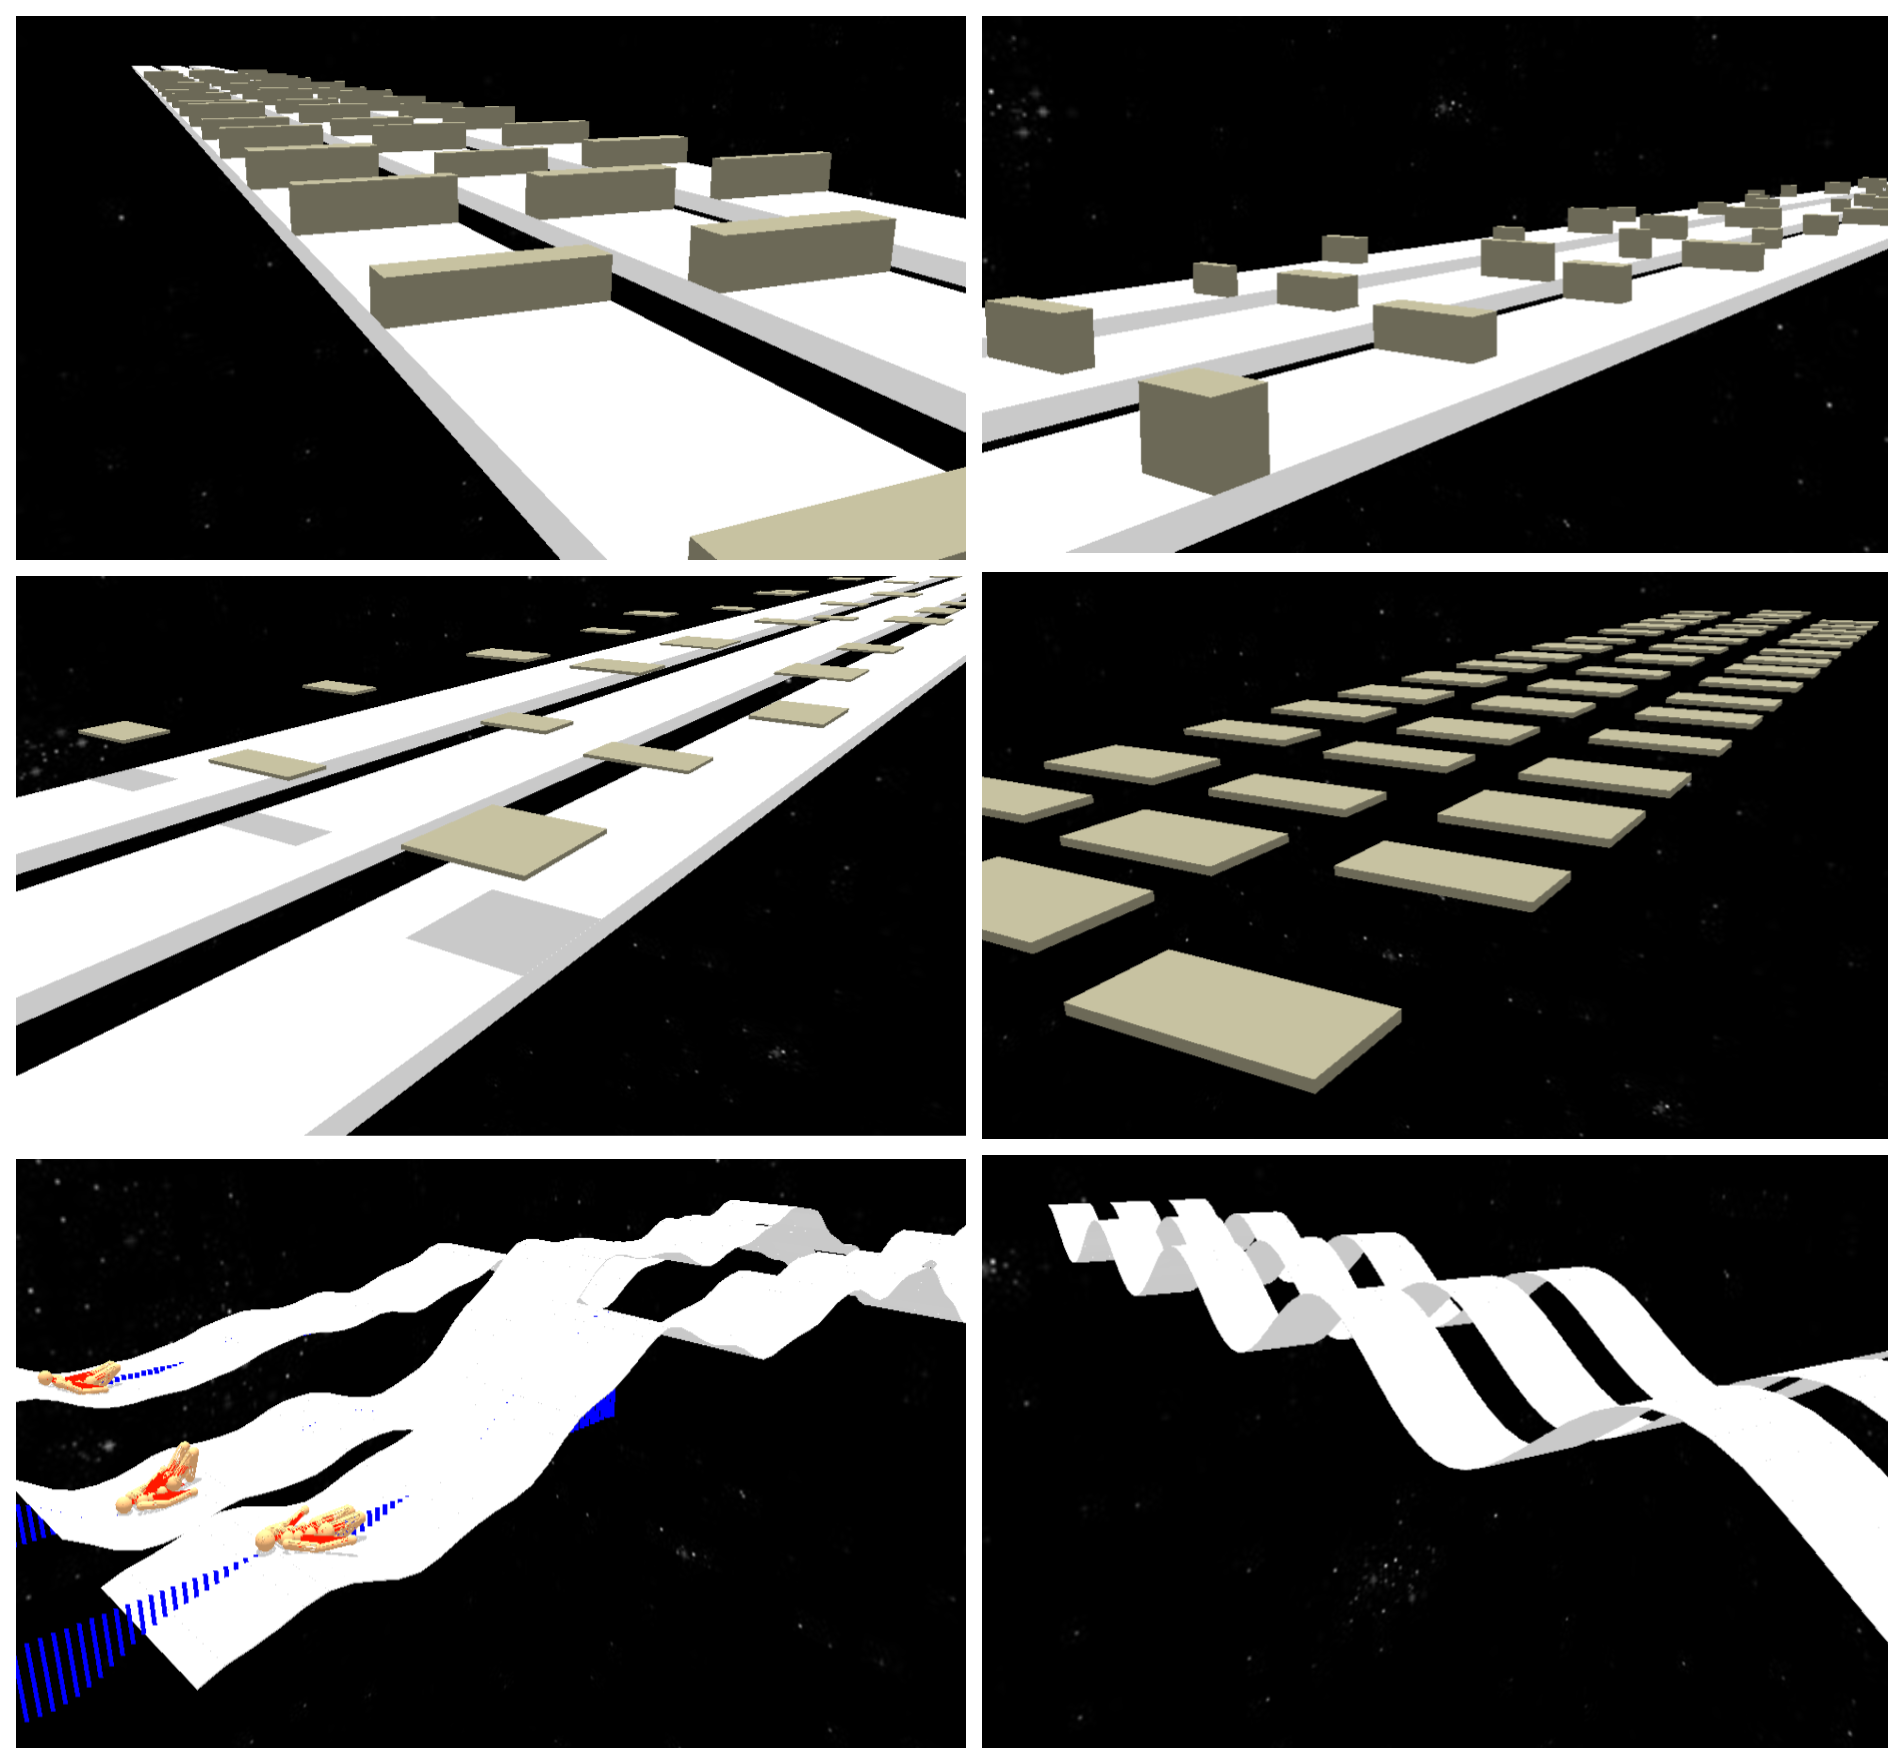
\includegraphics[width=0.85\linewidth]{_imgs/img_tysocmjc_terrains.png}
    \caption{Procedural Terrain Generators}
\end{figure}

\begin{figure}
    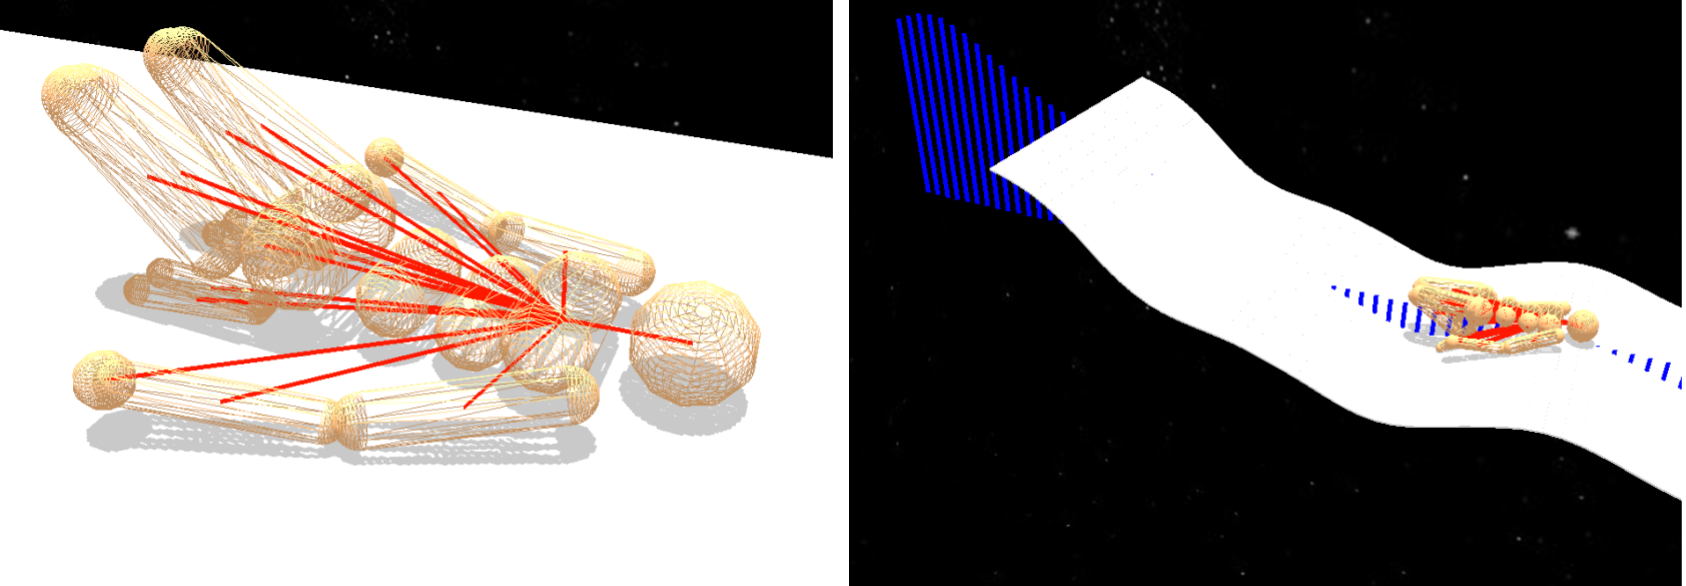
\includegraphics[width=0.85\linewidth]{_imgs/img_tysocmjc_sensors.png}
    \caption{Sensor types: intrinsic(left), extrinsic(right)}
\end{figure}

\begin{block}{Roadmap}

\begin{itemize}
    \item \textbf{More environments, utilities and creation tools}
    \item \textbf{Full Bullet and DART support}
    \item \textbf{Python API and documentation}
\end{itemize}

\end{block}

\setbeamercolor{block alerted title}{fg=black,bg=norange} % Change the alert block title colors
\setbeamercolor{block alerted body}{fg=black,bg=white} % Change the alert block body colors

\begin{block}{References}

\begin{itemize}
\item (1) Bellemare, et al. \textit{The Arcade Learning Environment}. JAIR 2013.
\item (2) Shane Legg, Marcus Hutter. \textit{Universal Intelligence}. ArXiv 2017.
\item (3) Yuval Tassa, et al. \textit{DeepMind Control Suite}. ArXiv 2018.
\item (4) Glen Berseth, et al. \textit{Terrain RL Simulator}. ArXiv 2018.
\item (5) Linxi Fan, Yuke Zhu, et al. \textit{SURREAL}. CoRL 2018.
\item (6) Yan Duan, Xi Chen, et al. \textit{Bencmarking DeepRL for Continuous Control}. ICML 2016.
\end{itemize}

\end{block}


%----------------------------------------------------------------------------------------

\end{column} % End of the third column

\end{columns} % End of all the columns in the poster

\end{frame} % End of the enclosing frame

\end{document}
